\begin{spacing}{1}
    \chapter*{Abstract}
\end{spacing}
\begin{wrapfigure}{r}{0.3\textwidth}
    \begin{center}
      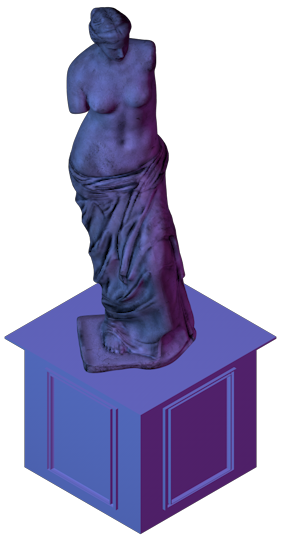
\includegraphics[width=0.2\textwidth]{pics/statue.png}
    \end{center}
\end{wrapfigure}
% TODO ask wegen Abstract bei Frontend
\emph{3D Portfolio Gallery – Server} is the back end of the application 3D Portfolio Gallery, which was developed by Litzlbauer Lorenz and Maar Fabian.
Thanks to it, designers get the possibility to upload their work online, where it gets displayed in a three-dimensional room.


The server is developed by Halilovic Ema and provides an interface to provide the front end with all the needed data. 
This data is saved in a database, which also enables file upload. 
The programmed interfaces are secured by a token system.


The technology used to build the server was Quarkus, along with a PostgreSQL database.
For token management, JSON Web Tokens were used.
\newpage
\begin{spacing}{1}
    \chapter*{Zusammenfassung}
\end{spacing}
\begin{wrapfigure}{r}{0.3\textwidth}
    \begin{center}
      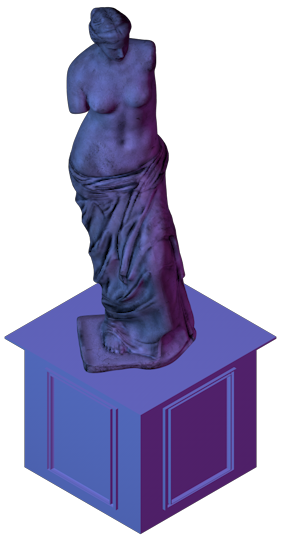
\includegraphics[width=0.2\textwidth]{pics/statue.png}
    \end{center}
\end{wrapfigure}
\emph{3D Portfolio Gallery – Server} ist das Backend der Applikation 3D Portfolio Gallery, welche von Litzlbauer Lorenz und Maar Fabian programmiert wurde. 
Sie bietet Designenden eine Möglichkeit, eigene Werke innerhalb eines dreidimensionalen Raumes auszustellen. 


Der Server wurde von Halilovic Ema erstellt und bietet der vorher erwähnten Arbeit Schnittstellen, um alle Daten abrufen zu können. 
Die dafür benötigten Daten sind auf einer Datenbank gesichert. 
Dank dieser wird ebenso das Hochladen von Dateien ermöglicht.  
Die ausprogrammierten Schnittstellen werden durch ein Token-System verschlüsselt. 


Die, für den Aufbau des Servers verwendete Technologie, ist Quarkus, gemeinsam mit einer PostgreSQL-Datenbank.
Für die Token-Verwaltung werden JSON Web Token verwendet.

